\documentclass[ucs,9pt]{beamer}

% Copyright 2004 by Till Tantau <tantau@users.sourceforge.net>.
%
% In principle, this file can be redistributed and/or modified under
% the terms of the GNU Public License, version 2.
%
% However, this file is supposed to be a template to be modified
% for your own needs. For this reason, if you use this file as a
% template and not specifically distribute it as part of a another
% package/program, I grant the extra permission to freely copy and
% modify this file as you see fit and even to delete this copyright
% notice.
%
% Modified by Tobias G. Pfeiffer <tobias.pfeiffer@math.fu-berlin.de>
% to show usage of some features specific to the FU Berlin template.

% remove this line and the "ucs" option to the documentclass when your editor is not utf8-capable
\usepackage[utf8x]{inputenc}    % to make utf-8 input possible
\usepackage[english]{babel}     % hyphenation etc., alternatively use 'german' as parameter

% Template for talks using the Corporate Design of the Freie Universitaet
%   Berlin, created following the guidelines on www.fu-berlin.de/cd by
%   Tobias G. Pfeiffer, <tobias.pfeiffer@math.fu-berlin.de>
% This file can be redistributed and/or modified in any way you like.
%   If you feel you have done significant improvements to this template,
%   please consider providing your modified version to
%   https://www.mi.fu-berlin.de/w/Mi/BeamerTemplateCorporateDesign

\usepackage{amsmath,dsfont,listings}

%%% FU logo
% small version for upper right corner of normal pages
\pgfdeclareimage[height=0.9cm]{university-logo}{FULogo_RGB}
\logo{\pgfuseimage{university-logo}}
% large version for upper right corner of title page
\pgfdeclareimage[height=1.085cm]{big-university-logo}{FULogo_RGB}
\newcommand{\titleimage}[1]{\pgfdeclareimage[height=2.92cm]{title-image}{#1}}
%\titlegraphic{\pgfuseimage{title-image}}
%%% end FU logo

% NOTE: 1cm = 0.393 in = 28.346 pt;    1 pt = 1/72 in = 0.0352 cm
\setbeamersize{text margin right=3.5mm, text margin left=7.5mm}  % text margin

% colors to be used
\definecolor{text-grey}{rgb}{0.45, 0.45, 0.45} % grey text on white background
\definecolor{bg-grey}{rgb}{0.66, 0.65, 0.60} % grey background (for white text)
\definecolor{fu-blue}{RGB}{0, 51, 102} % blue text
\definecolor{fu-green}{RGB}{153, 204, 0} % green text
\definecolor{fu-red}{RGB}{204, 0, 0} % red text (used by \alert)

% switch off the sidebars
% TODO: loading \useoutertheme{sidebar} (which is maybe wanted) also inserts
%   a sidebar on title page (unwanted), also indents the page title (unwanted?),
%   and duplicates the navigation symbols (unwanted)
\setbeamersize{sidebar width left=0cm, sidebar width right=0mm}
\setbeamertemplate{sidebar right}{}
\setbeamertemplate{sidebar left}{}
%    XOR
% \useoutertheme{sidebar}

% frame title
% is truncated before logo and splits on two lines
% if neccessary (or manually using \\)
\setbeamertemplate{frametitle}{%
    \vskip-30pt \color{text-grey}\large%
    \begin{minipage}[b][23pt]{80.5mm}%
    \flushleft\insertframetitle%
    \end{minipage}%
}

%%% title page
% TODO: get rid of the navigation symbols on the title page.
%   actually, \frame[plain] *should* remove them...
\setbeamertemplate{title page}{
% upper right: FU logo
\vskip2pt\hfill\pgfuseimage{big-university-logo} \\
\vskip6pt\hskip3pt
% title image of the presentation
\begin{minipage}{11.6cm}
\hspace{-1mm}\inserttitlegraphic
\end{minipage}

% set the title and the author
\vskip14pt
\parbox[top][1.35cm][c]{11cm}{\color{text-grey}\inserttitle \\ \small \insertsubtitle}
\vskip11pt
\parbox[top][1.35cm][c]{11cm}{\small \insertauthor \\ \insertinstitute \\[3mm] \insertdate}
}
%%% end title page

%%% colors
\usecolortheme{lily}
\setbeamercolor*{normal text}{fg=black,bg=white}
\setbeamercolor*{alerted text}{fg=fu-red}
\setbeamercolor*{example text}{fg=fu-green}
\setbeamercolor*{structure}{fg=fu-blue}

\setbeamercolor*{block title}{fg=white,bg=black!50}
\setbeamercolor*{block title alerted}{fg=white,bg=black!50}
\setbeamercolor*{block title example}{fg=white,bg=black!50}

\setbeamercolor*{block body}{bg=black!10}
\setbeamercolor*{block body alerted}{bg=black!10}
\setbeamercolor*{block body example}{bg=black!10}

\setbeamercolor{bibliography entry author}{fg=fu-blue}
% TODO: this doesn't work at all:
\setbeamercolor{bibliography entry journal}{fg=text-grey}

\setbeamercolor{item}{fg=fu-blue}
\setbeamercolor{navigation symbols}{fg=text-grey,bg=bg-grey}
%%% end colors

%%% headline
\setbeamertemplate{headline}{
\vskip4pt\hfill\insertlogo\hspace{3.5mm} % logo on the right

\vskip6pt\color{fu-blue}\rule{\textwidth}{0.4pt} % horizontal line
}
%%% end headline

%%% footline
\newcommand{\footlinetext}{\insertshortinstitute, \insertshorttitle, \insertshortdate}
\setbeamertemplate{footline}{
\vskip5pt\color{fu-blue}\rule{\textwidth}{0.4pt}\\ % horizontal line
\vskip2pt
\makebox[123mm]{\hspace{7.5mm}
\color{fu-blue}\footlinetext
\hfill \raisebox{-1pt}{\usebeamertemplate***{navigation symbols}}
\hfill \insertframenumber}
\vskip4pt
}
%%% end footline

%%% settings for listings package
\lstset{extendedchars=true, showstringspaces=false, basicstyle=\footnotesize\sffamily, tabsize=2, breaklines=true, breakindent=10pt, frame=l, columns=fullflexible}
\lstset{language=Java} % this sets the syntax highlighting
\lstset{mathescape=true} % this switches on $...$ substitution in code
% enables UTF-8 in source code:
\lstset{literate={ä}{{\"a}}1 {ö}{{\"o}}1 {ü}{{\"u}}1 {Ä}{{\"A}}1 {Ö}{{\"O}}1 {Ü}{{\"U}}1 {ß}{\ss}1}
%%% end listings  % THIS is the line that includes the FU template!


\usepackage{arev,t1enc} % looks nicer than the standard sans-serif font
% if you experience problems, comment out the line above and change
% the documentclass option "9pt" to "10pt"



\usepackage{svg}
\usepackage{amsmath}
\beamertemplatenavigationsymbolsempty


\title{Cryptography presentation}

\subtitle{As part of the lecture \textit{Kryptographie und Sicherheit in Verteilten Systemen}}

\author{L.~Herich \and A.~Plötze}

\institute[FU Berlin]{Freie Universität Berlin}

\date{Berlin, 2015}
\subject{Kryptographie Präsentation}
\renewcommand{\footlinetext}{\insertshortinstitute, \insertshorttitle, \insertshortdate}


\begin{document}

\begin{frame}[plain]
  \titlepage
\end{frame}

\begin{frame}{Outline}
  \tableofcontents
  % You might wish to add the option [pausesections]
\end{frame}


\section{Lecture content}

\begin{frame}{Git repository with topics of the lecture}
    \begin{figure}[h]
        \centering
        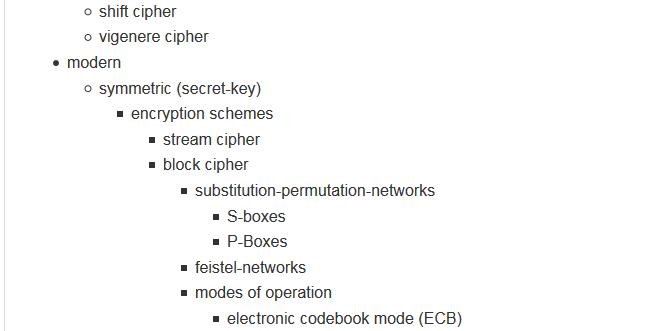
\includegraphics[width=0.5\textwidth]{figures/list_of_content.png}
        \caption{Git repository with the summarized topics of the lecture}
    \end{figure}
    \begin{block}{Fork it on github.com}
        \begin{itemize}
            \item 
            \url{https://github.com/lherich/cryptography}
            \item
            \url{git@github.com:lherich/cryptography.git}
        \end{itemize}
    \end{block}
\end{frame}


%
% Encryption schemes
%
\section{Encryption schemes}
\begin{frame}
    \centering
    \huge{Encryption schemes}
\end{frame}


% Eavesdropping (EAV)
\subsection{Eavesdropping (EAV)}

\begin{frame}{Eavesdropping (EAV)}
    \begin{block}{The adversarial indistinguishability experiment $PrivK_{A,\Pi}^{EAV}$}
        $\Pi = (Gen, Enc, Dec)$ is any private-key encryption scheme, $A$ is the adversary, $M$ message space, $n$ is the security paramter\\
        
        \begin{enumerate}
            \item $(m_0,m_1) \in M \leftarrow A$
            \item $k \overset{\$}{\leftarrow} Gen(1^n)$
            \item $b \overset{\$}{\leftarrow} \{0,1\}$
            \item c is given to A
            \item $b' \leftarrow A$
            \item $c \leftarrow Enc_{k}(m_b)$
                \item $if(b = b')\ output\ 1$ \\
                $else\ output\ 0$
        \end{enumerate}
        
        indistinguishable encryptions in the presence of an eavesdropper: if for all probabilistic polynomial-time adversaries $A$:\\
        $Pr[PrivK_{A,\Pi}^{EAV}(n) = 1] \leq \frac{1}{2} + negl(n)$
        $\Leftrightarrow \left | Pr[output(PrivK_{A,\Pi}^{EAV}) = 1] - Pr[output(PrivK_{A,\Pi}^{EAV}(n,1) = 1)] \right | \leq negl(n)$
    \end{block}
\end{frame}

\begin{frame}{Eavesdropping (EAV)}
    
    \begin{figure}[h]
        \centering
        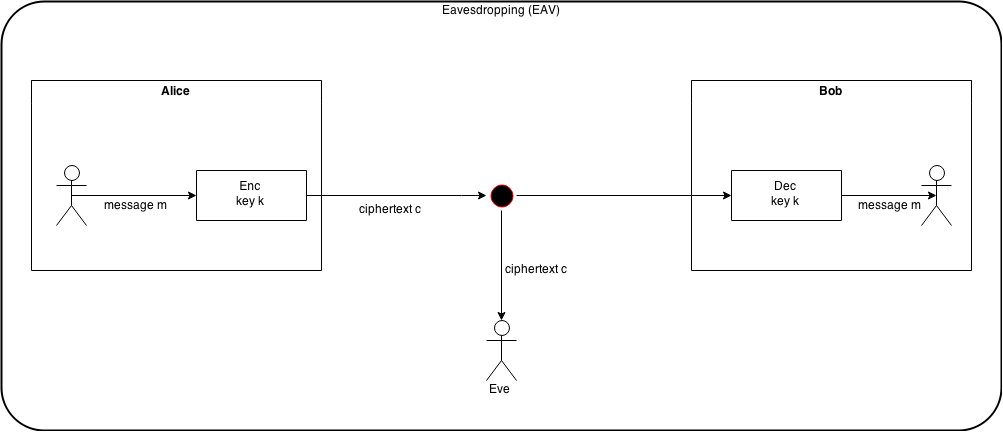
\includegraphics[width=0.8\textwidth]{figures/EAV.png}
        \caption{Eavesdropping (EAV)}
    \end{figure}
    IND-EAV can be constructed by a PRG\footnote{Katz and Lindell: Introduction to Modern Cryptography, 2007 p. 73}
\end{frame}


% Known-plaintext attack (KPA)
\subsection{Known-plaintext attack (KPA)}
    
\begin{frame}{Known-plaintext attack (KPA)}
    
    \begin{figure}[h]
        \centering
        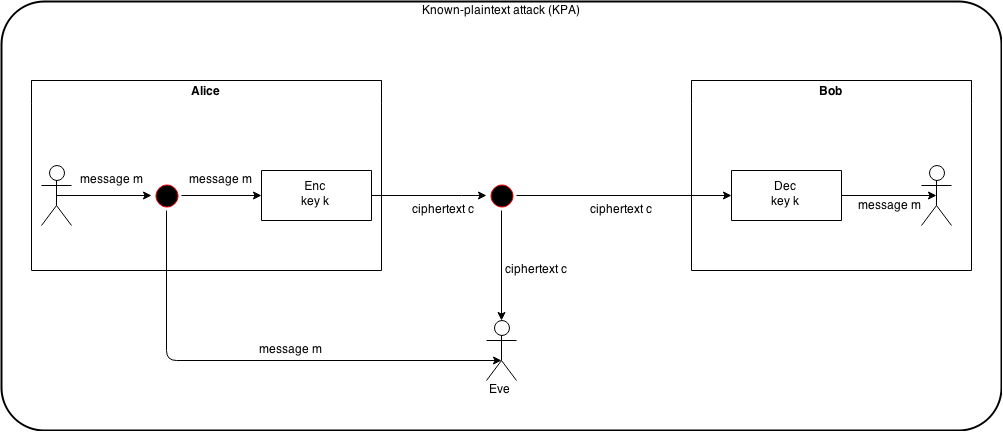
\includegraphics[width=0.8\textwidth]{figures/KPA.png}
        \caption{Known-plaintext attack (KPA)}
    \end{figure}
\end{frame}


% Chosen-plaintext attack (CPA)
\subsection{Chosen-plaintext attack (CPA)}

\begin{frame}{Chosen-plaintext attack (CPA)}
    \begin{block}{The CPA indistinguishability experiment $PrivK_{A,\Pi}^{CPA}(n)$:}
        $\Pi = (Gen, Enc, Dec)$ is any private-key encryption scheme\\
        $A$ is the adversary\\
        $n$ is the security paramter\\
        
        \begin{enumerate}
            \item $k \overset{\$}{\leftarrow} Gen(1^n)$
            \item $(m_{0},m_{1}) \leftarrow A^{Enc_{k}(.)}(1^{n})$
            \item $b \overset{\$}{\leftarrow} \{0,1\}$
            \item $c \leftarrow Enc_{k}(m_{b})$
            \item c is given to A
            \item $b' \leftarrow A^{Enc_{k}(.)}(c)$
            \item $if(b = b')\ output\ 1$ \\
            $else\ output\ 0$
        \end{enumerate}
        
        CPA-secure: if for all probabilistic polynomial-time adversaries $A$:\\
        $Pr[PrivK_{A,\Pi}^{CPA}(n) = 1] \leq \frac{1}{2} + negl(n)$
    \end{block}
\end{frame}

\begin{frame}{Chosen-plaintext attack (CPA)}
    
    \begin{figure}[h]
        \centering
        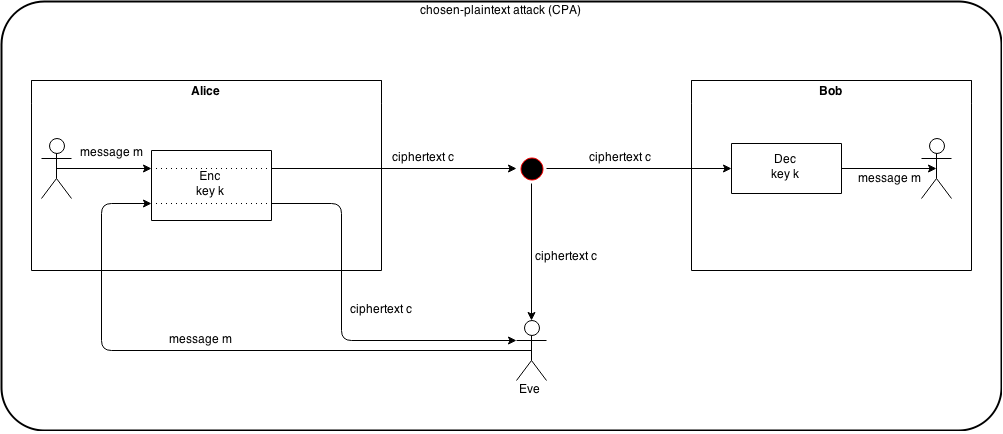
\includegraphics[width=0.8\textwidth]{figures/CPA.png}
        \caption{Chosen-plaintext attack (CPA)}
    \end{figure}
    IND-CPA can be constructed by a PRF\footnote{Katz and Lindell: Introduction to Modern Cryptography, 2007 p. 89}
\end{frame}



% Chosen-ciphertext attack (CCA)
\subsection{Chosen-ciphertext attack (CCA)}
\begin{frame}{Chosen-ciphertext attack (CCA)}
    \begin{block}{The CCA indistinguishability experiment $ PrivK_{A,\Pi}^{cca}(n) $}
        $\Pi = (Gen, Enc, Dec)$ is any private-key encryption scheme\\
        $A$ is the adversary\\
        $n$ is the security paramter\\
        \begin{enumerate}
            \item $k \overset{\$}{\leftarrow} Gen(1^n)$
            \item $(m_{0},m_{1}) \leftarrow A^{Enc_{k}(.), Dec_{k}(.)}(ask, 1^{n})$
            \item $b \overset{\$}{\leftarrow} \{0, 1\}$
            \item $c \leftarrow Enc_{k}(m_{b})$
            \item $b' \leftarrow A^{Enc_{k}(.), Dec_{k}(.)}(guess, c)$
            \item $if(b = b')\ output\ 1$ \\
            $else\ output\ 0$
        \end{enumerate}
        CCA-secure: if for all probabilistic polynomial-time adversaries $A$:\\
        $ PrivK_{A,\Pi}^{cca}(n) = 1 \leq \frac{1}{2} + negl(n) $
    \end{block}
\end{frame}

\begin{frame}{Chosen-ciphertext attack (CCA)}
    
    \begin{figure}[h]
        \centering
        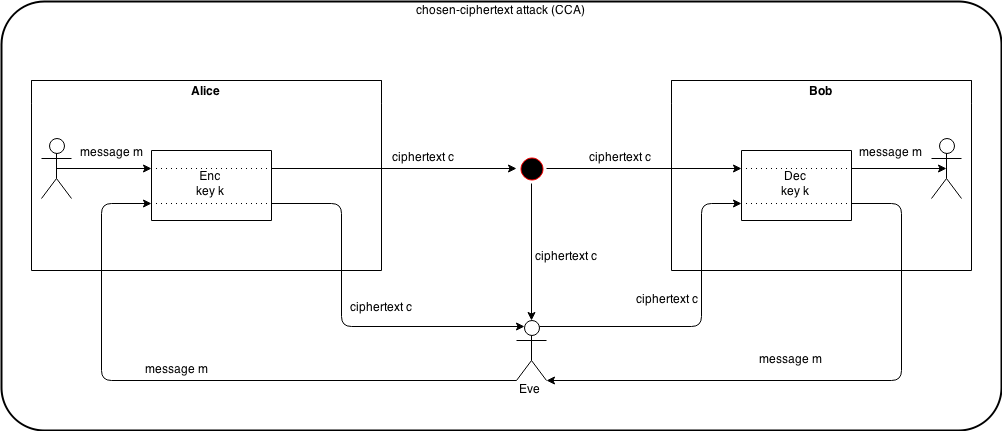
\includegraphics[width=0.8\textwidth]{figures/CCA.png}
        \caption{Chosen-ciphertext attack (CCA)}
    \end{figure}
    CBC, OFB and CTR-Mode are not CCA2-secure encryption schemes for every F (see assignment 6).\\
    CCA1/CCA2 can be constructed by a PRF\\
\end{frame}


%
% Signature schemes
%
\section{Signature schemes}

\begin{frame}
    \centering
    \huge{Signature schemes}
\end{frame}

% Adaptive-chosen-message attack (ACMA)
\subsection{Adaptive-chosen-message attack (ACMA)}

\begin{frame}{Adaptive-chosen-message attack (ACMA)}
    \begin{block}{The message authentication experiment Mac-forge$_{A,\Pi}(n)$}
        \begin{enumerate}
            \item $k \overset{\$}{\leftarrow} \{0,1\}^n$
            \item $(m, t) \leftarrow A^{Mac_{k}}(1^{n})$
            \item $if(m \notin Q\ and\ Vrfy_{k}(m, t) = 1)\ output\ 1$\\
            $otherwise\ output\ 0$
        \end{enumerate}
        
        A MAC-scheme Pi is secure against adaptive-chosen-message-attacks, if for all probabilistic polynomial-time adversaries A, there exists a negligible function negl, such that:\\
        $Pr[Mac-force_{A,\Pi}(n) = 1] \leq negl(n)$
    \end{block}
\end{frame}

\begin{frame}{Adaptive-chosen-message attack (ACMA)}
    \begin{figure}[h]
        \centering
        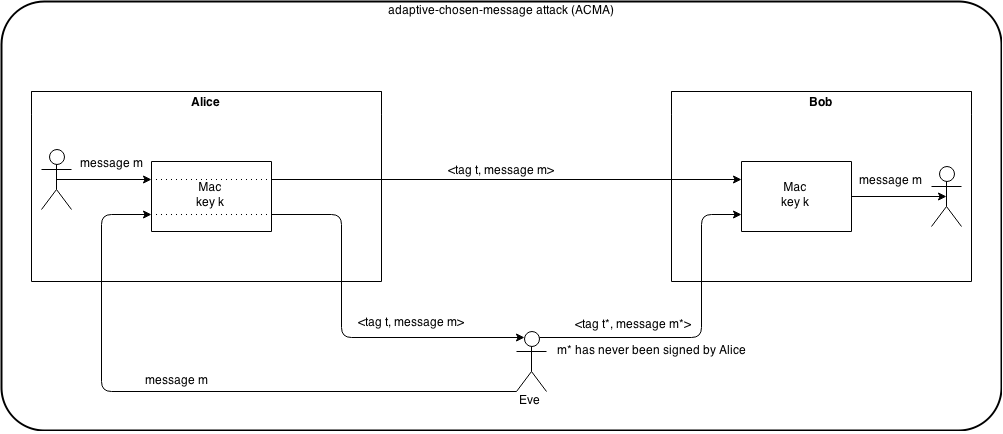
\includegraphics[width=0.8\textwidth]{figures/ACMA.png}
        \caption{Adaptive-chosen-message attack (ACMA)}
    \end{figure}
\end{frame}


\section*{Questions}

\begin{frame}{Questions}
    \huge{Any annotations or questions?}
\end{frame}
\end{document}
